%=================================================================
% MIT LICENSE
%=================================================================
% Copyright (c) 2022 Techneatium
%
% Permission is hereby granted, free of charge, to any person obtaining a copy
% of this software and associated documentation files (the "Software"), to deal
% in the Software without restriction, including without limitation the rights
% to use, copy, modify, merge, publish, distribute, sublicense, and/or sell
% copies of the Software, and to permit persons to whom the Software is
% furnished to do so, subject to the following conditions:
%
% The above copyright notice and this permission notice shall be included in all
% copies or substantial portions of the Software.
%
% THE SOFTWARE IS PROVIDED "AS IS", WITHOUT WARRANTY OF ANY KIND, EXPRESS OR
% IMPLIED, INCLUDING BUT NOT LIMITED TO THE WARRANTIES OF MERCHANTABILITY,
% FITNESS FOR A PARTICULAR PURPOSE AND NONINFRINGEMENT. IN NO EVENT SHALL THE
% AUTHORS OR COPYRIGHT HOLDERS BE LIABLE FOR ANY CLAIM, DAMAGES OR OTHER
% LIABILITY, WHETHER IN AN ACTION OF CONTRACT, TORT OR OTHERWISE, ARISING FROM,
% OUT OF OR IN CONNECTION WITH THE SOFTWARE OR THE USE OR OTHER DEALINGS IN THE
% SOFTWARE.
%=================================================================

%-----------------------------------------------------------------
% BEGIN DOCUMENT
%-----------------------------------------------------------------
\documentclass[fontHelvetica]{TechCheck}
\title{AH64_Cheatsheet}
\author{Techneatium}

\setaircraftlong{AH-64D AIRCRAFT} % sets long label for title page
\setaircraftshort{AH-64D} % sets short label for header
\settabnumber{8} % sets number of tabs for document

% spacing within lists
% \setlist[enumerate, 1]{leftmargin=1.5em, itemsep=1pt, parsep=0pt, label=(\alph*)}
% \setlist[enumerate, 2]{leftmargin=1.5em, itemsep=1pt, parsep=0pt}
% \setlist[itemize, 1]{leftmargin=1.5em, itemsep=1pt, parsep=0pt, label=\textbf{\textbullet}}
% \setlist[itemize, 2]{leftmargin=1.5em, itemsep=1pt, parsep=0pt}


\begin{document}
	%-----------------------------------------------------------------
% TITLE PAGE
%-----------------------------------------------------------------
	% deactivate header and footer
	\pagestyle{empty}
	\newlength{\centeroffset}
	\setlength\centeroffset{(\chevin-\outmar-0.5cm)/2}
	\begin{tikzpicture}[overlay, remember picture]
	\node[
	]() at ([xshift=\centeroffset,yshift=8.5cm]current page.center) {
		\Huge \titlefont\textbf{Pocket Checklist}
	};
	\node[
	]() at ([xshift=\centeroffset,yshift=7cm]current page.center) {
		\resizebox{10cm}{!}{\titlefont\textbf{\colorbox{color1}{\textcolor{white}{\aircraftlong}}}}
	};
	\node[
	]() at ([xshift=\centeroffset,yshift=5.5cm]current page.center) {
		\Large \titlefont\textbf{\colorbox{color1}{\textcolor{white}{REV: \today}}} \blue{}
	};
	\node[
	]() at ([xshift=\centeroffset,yshift=-1cm]current page.center) {
		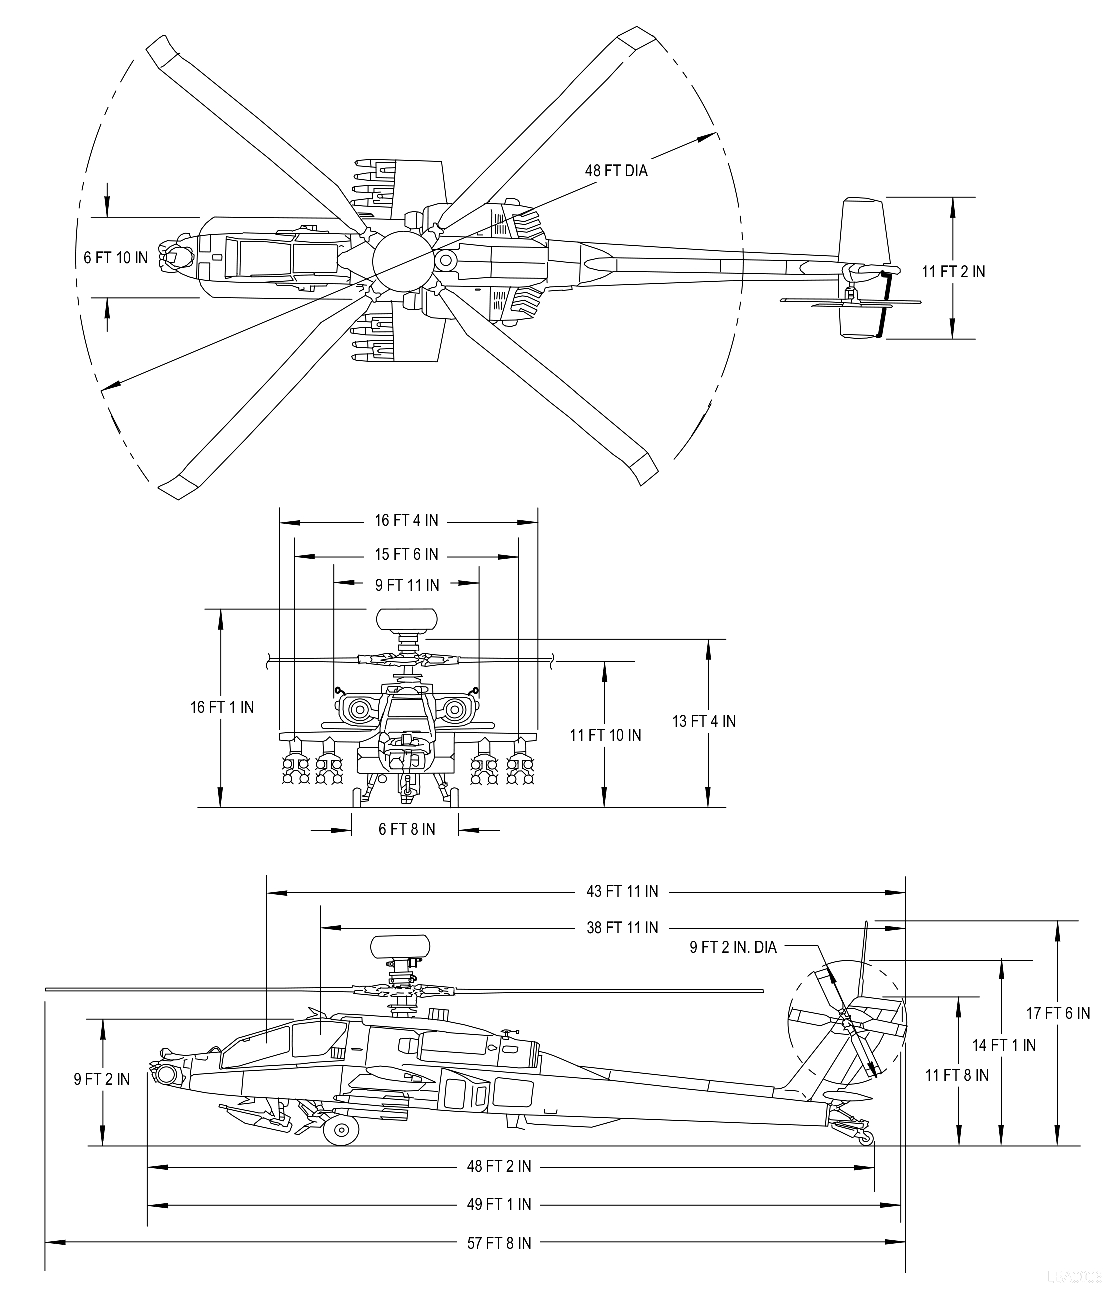
\includegraphics[
			width=0.75\linewidth,
			% page = {1},
			% trim = {3cm, 10.5cm, 6.5cm, 13.5cm},
			% clip
		]{Apache_dimensions.pdf}
	};
	% Black area for white chevrons
	\fill[color1]
		([xshift=\outmar, yshift=0.2cm]current page text area.north east) --
		([xshift=\outmar, yshift=-\botmar]current page text area.south east) --
		([xshift=\chevin-0.5cm, yshift=-\botmar]current page text area.south east) --
		([xshift=\chevin-0.5cm, yshift=0.2cm]current page text area.north east) --
		cycle;
	\end{tikzpicture}
	% label for hyperrefs back to frontpage
	\label{frontpage}
	% make chevrons
	\thumbfront{Procedures}{0}
	% \thumbfront{Systems}{1}
	% % use tabular for multi line node
	% \thumbfront{\begin{tabular}{c} APG-68 \\ FCR \end{tabular}}{2}
	% \thumbfront{\begin{tabular}{c} LITENING \\ TGP \end{tabular}}{3}
	% \thumbfront{\begin{tabular}{c} A/G \\ Weapons \end{tabular}}{4}
	% \thumbfront{\begin{tabular}{c} A/A \\ Weapons \end{tabular}}{5}
	\thumbwide

	\clearpage
	\null\vspace{0cm}

	\begin{tcolorbox}[
		enhanced, colback=white, colframe=color1, colbacktitle=white, coltitle=color1, sharp corners, attach boxed title to top center={yshift=2mm},
		boxed title style={
			sharp corners,
			drop shadow=color1!100
		}, title=\LARGE\textbf{DISCLAIMER}
	]
		\textbf{This document represents a personal project and is intended for entertainment purposes only. Do not use for training purposes or in real life scenarios.}
	\end{tcolorbox}

	\cleardoublepage

	\thumbnar
	\dominitoc
	\tableofcontents
	\cleardoublepage

	% restart page counter
	\setcounter{page}{1}
	% reactivate header and footer
	\pagestyle{body}

	\chapter{PROCEDURES}
	\thumbtab{Procedures}{0}
	\minitoc
	\cleardoublepage

	\section{START-UP}

	\subsection{INTERIOR CHECKS}
	\begin{center}
		\begin{longtable}{l p{3cm} | p{8cm}}
			\toprule
			\textbf{\textbullet} & \blue{Canopy Door} \textbf{(PLT/CPG)} & \textbf{As Desired} \\
			\midrule
			\multicolumn{3}{c}{\blue{LEFT SIDE -- BACK TO FRONT}} \\
			\midrule
			\textbf{\textbullet} & \blue{Lights Panel} \textbf{(PLT/CPG)}  &
			\begin{minipage}[t]{\linewidth}
				\begin{itemize}
					\item \textbf{EXT LT/INTR LT Panel} \dotfill \textbf{As Required} \\
					\emph{(PLT)}
					\item \textbf{INTR LT Panel} \dotfill \textbf{As Required} \\
					\emph{(CPG)}
				\end{itemize}
			\end{minipage} \\
			\midrule
			\textbf{\textbullet} & \blue{Power Levers} \textbf{(PLT/CPG)} & \textbf{OFF} \\
			\midrule
			\textbf{\textbullet} & \blue{ENG START Switches} \textbf{(PLT)} & \textbf{OFF} \\
			\midrule
			\textbf{\textbullet} & \blue{RTR BRK Switch} \textbf{(PLT)} & \textbf{OFF} \\
			\midrule
			\textbf{\textbullet} & \blue{NVS MODE Switch} \textbf{(PLT/CPG)} & \textbf{OFF} \\
			\midrule
			\multicolumn{3}{c}{\blue{FRONT PANEL -- LEFT TO RIGHT}} \\
			\midrule
			\textbf{\textbullet} & \blue{KU Brightness Knob} \textbf{(PLT/CPG)} & \textbf{As Desired} \\
			\midrule
			\textbf{\textbullet} & \blue{VIDEO Panel} \textbf{(PLT)} & \textbf{Knobs at 12 o'clock} \\
			\midrule
			\textbf{\textbullet} & \blue{MPD/EUFD Brightness Knob} \textbf{(PLT/CPG)} & \textbf{As Desired} \\
			\midrule
			\textbf{\textbullet} & \blue{CMWS} \textbf{(PLT)} &
			\begin{minipage}[t]{\linewidth}
				\begin{itemize}
					\item \textbf{CMWS Control Indicator PWR} \dotfill \textbf{OFF}
					\item \textbf{CMWS/NAV Switch} \dotfill \textbf{CMWS}
					\item \textbf{BYPASS/AUTO Switch} \dotfill \textbf{AUTO}
					\item \textbf{JETTISON Switch} \dotfill \textbf{OFF}
				\end{itemize}
			\end{minipage} \\
			\midrule
			\textbf{\textbullet} & \blue{TEDAC R Grip LT} \textbf{(CPG)} & \textbf{OFF} \\
			\midrule
			\textbf{\textbullet} & \blue{PARK BRAKE} \textbf{(PLT)} & \textbf{SET}, Handle out \\
			\midrule
			\textbf{\textbullet} & \blue{Standby Instruments} \textbf{(PLT)} & \textbf{Check}, caged \\
			\midrule
			\multicolumn{3}{c}{\blue{RIGHT SIDE -- FRONT TO BACK}} \\
			\midrule
			\textbf{\textbullet} & \blue{COMM Panel} \textbf{(PLT/CPG)} & \textbf{As Desired} \\
			\midrule
			\textbf{\textbullet} & \blue{HDU} \textbf{(PLT/CPG)} & \textbf{As Desired} \\
			\bottomrule
		\end{longtable}
	\end{center}

	\begin{enumerate}[leftmargin=0.1\linewidth,rightmargin=0.1\linewidth]
		\item \blue{Canopy Door} \textbf{(PLT/CPG)} \dotfill \textbf{As Desired}
		\item \blue{Lights Panel} \textbf{(PLT/CPG)} 
		\begin{itemize}
			\item \textbf{EXT LT/INTR LT Panel} \dotfill \textbf{As Required}
			\emph{(PLT)}
			\item \textbf{INTR LT Panel} \dotfill \textbf{As Required}
			\emph{(CPG)}
		\end{itemize}
		\item \blue{Power Levers} \textbf{(PLT/CPG)} \dotfill \textbf{OFF}
		\item \blue{ENG START Switches} \textbf{(PLT)} \dotfill \textbf{OFF}
		\item \blue{RTR BRK Switch} \textbf{(PLT)} \dotfill \textbf{OFF}
		\item \blue{NVS MODE Switch} \textbf{(PLT/CPG)} \dotfill \textbf{OFF}
		\item \blue{KU Brightness Knob} \textbf{(PLT/CPG)} \dotfill \textbf{As Desired}
		\item \blue{VIDEO Panel} \textbf{(PLT)} \dotfill \textbf{Knobs at 12 o'clock}
		\item \blue{MPD/EUFD Brightness Knob} \textbf{(PLT/CPG)} \dotfill \textbf{As Desired}
		\item \blue{CMWS} \textbf{(PLT)}
		\begin{itemize}
				\item \textbf{CMWS Control Indicator PWR} \dotfill \textbf{OFF}
				\item \textbf{CMWS/NAV Switch} \dotfill \textbf{CMWS}
				\item \textbf{BYPASS/AUTO Switch} \dotfill \textbf{AUTO}
				\item \textbf{JETTISON Switch} \dotfill \textbf{OFF}
		\end{itemize}
		\item \blue{TEDAC R Grip LT} \textbf{(CPG)} \dotfill \textbf{OFF}
		\item \blue{PARK BRAKE} \textbf{(PLT)} \dotfill \textbf{SET}, Handle out
		\item \blue{Standby Instruments} \textbf{(PLT)} \dotfill \textbf{Check}, caged
		\item \blue{COMM Panel} \textbf{(PLT/CPG)} \dotfill \textbf{As Desired}
		\item \blue{HDU} \textbf{(PLT/CPG)} \dotfill \textbf{As Desired} \\
	\end{enumerate}

	\clearpage

	\subsection{APU-START}
	\begin{center}
		\begin{longtable}{l p{3cm} | p{8cm}}
			\toprule
			\multicolumn{3}{c}{\blue{PRE APU START}} \\
			\midrule
			1. & \blue{MSTR IGN Switch} \textbf{(PLT)} & \textbf{BATT} \\
			\midrule
			2. & \blue{Searchlight} \textbf{(PLT)} & \textbf{As Required} \\
			\midrule
			3. & \blue{TAIL WHEEL Button} \textbf{(PLT)} & \textbf{Locked}, UNLOCKED Light is off \\
			\midrule
			4. & \blue{EMERG HYD Button} \textbf{(PLT/CPG)} & Verify \textbf{ON Light} not illuminated \\
			\midrule
			5. & \blue{Cautions} \textbf{(PLT/CPG)} & \textbf{Check MSTR WARN, MSTR CAUT, EUFD} \\
			\midrule
			6. & \blue{Fire Test} \textbf{(PLT/CPG)} &
			\begin{minipage}[t]{\linewidth}
				\begin{enumerate}
					\item \textbf{FIRE DET/EXTG TEST} \dotfill \textbf{Position 1} (PLT)
					\item \textbf{FIRE DET/EXTG TEST} \dotfill \textbf{Position 2} (CPG)
				\end{enumerate}
				\vspace{1em}
				\emph{In each position, both crewmembers should check the following}
				\begin{itemize}
					\item \textbf{MSTR WARN} \dotfill \textbf{illuminated}
					\item \textbf{ENG 1 FIRE} \dotfill \textbf{illuminated}
					\item \textbf{APU FIRE} \dotfill \textbf{illuminated}
					\item \textbf{ENG 2 FIRE} \dotfill \textbf{illuminated}
					\item \textbf{AFT DECK FIRE} \dotfill EUFD Warning
					\item \textbf{Voice Warning System} \dotfill activates
				\end{itemize}
			\end{minipage} \\
			\midrule
			\multicolumn{3}{c}{\blue{APU START}} \\
			\midrule
			7. & \blue{APU} \textbf{(PLT)} &
			\begin{minipage}[t]{\linewidth}
				\begin{enumerate}
					\item \textbf{APU Button} \dotfill \textbf{Press \& Release}
					\item \textbf{EUFD} \dotfill \textbf{Observe Advisories}
					\begin{itemize}
						\item \textbf{APU START}
						\item \textbf{APU POWER ON}
						\item \textbf{ACCUM OIL PRESS LO}
					\end{itemize}
				\end{enumerate}
			\end{minipage} \\
			\midrule
			\multicolumn{3}{c}{\blue{POST APU START}} \\
			\midrule
			8. & \blue{Canopy} \textbf{(PLT/CPG)} & \textbf{As Desired} \\
			\midrule
			9. & \blue{DTU Page} \textbf{(PLT/CPG)} & \textbf{Select Load} \\
			\midrule
			10. & \blue{Menu Page} \textbf{(PLT/CPG)} & \textbf{Perform DMS Sweep} \\
			\bottomrule
		\end{longtable}
	\end{center}

	\clearpage

	\subsection{DMS SWEEP}
	\notebox{
		\begin{itemize}
			\item \textbf{Recommended Technique: Clockwise from top right of any page}
			\item Exact sweep may vary based on mission requirements
		\end{itemize}
	}
	\begin{center}
		\begin{longtable}{l p{3cm} | p{8cm}}
			\toprule
			\textbf{\textbullet} & \blue{`M' Page} \textbf{(PLT/CPG)} &
			\begin{minipage}[t]{\linewidth}
				\begin{itemize}
					\item \textbf{ASE--UTIL}
					\begin{itemize}
						\item \textbf{RLWR VOICE} \dotfill \textbf{As Desired}
						\item \textbf{Chaff Settings} \dotfill \textbf{As Desired}
						\item \textbf{CHAFF Mode} \dotfill \textbf{As Desired}
					\end{itemize}
					\item \textbf{AUTOPAGE} \dotfill \textbf{As Desired}
				\end{itemize}
			\end{minipage} \\
			\midrule
			\textbf{\textbullet} & \blue{TSD Page} \textbf{(PLT/CPG)} &
			\begin{minipage}[t]{\linewidth}
				\begin{itemize}
					\item \textbf{SHOW}
					\begin{itemize}
						\item \textbf{PHASE} \dotfill \textbf{Select ATK}
						\item \textbf{THRT SHOW} \dotfill \textbf{As Desired}
						\item \textbf{COORD SHOW} \dotfill \textbf{As Desired}
						\item \textbf{PHASE} \dotfill \textbf{Select NAV}
						\item \textbf{COORD SHOW} \dotfill \textbf{As Desired}
					\end{itemize}
					\item \textbf{UTIL}
					\begin{itemize}
						\item \textbf{TIME} \dotfill \textbf{As Desired}
						\item \textbf{SYSTEM TIME} \dotfill \textbf{As Desired}
					\end{itemize}
					\item \textbf{SCALE} \dotfill \textbf{As Desired}
					\item \textbf{CTR} \dotfill \textbf{As Desired}
					\item \textbf{RTE}
					\begin{itemize}
						\item \textbf{DIR} \dotfill \textbf{Set Desired Point}
					\end{itemize}
					\item \textbf{MAP}
					\begin{itemize}
						\item \textbf{GRID} \dotfill \textbf{As Desired}
						\item \textbf{ORIENT} \dotfill \textbf{As Desired}
						\item \textbf{COLOR BAND} \dotfill \textbf{As Desired}
						\item \textbf{TYPE} \dotfill \textbf{As Desired}
					\end{itemize}
					\item \textbf{INST}
					\begin{itemize}
						\item \textbf{UTIL} \dotfill \textbf{Select}
						\item \textbf{ADF} \dotfill \textbf{ON} \\
						\hfill configure as necessary
					\end{itemize}
				\end{itemize}
			\end{minipage} \\
			\midrule
			\textbf{\textbullet} & \blue{WPN Page} \textbf{(PLT/CPG)} &
			\begin{minipage}[t]{\linewidth}
				\begin{itemize}
					\item \textbf{GRAYSCALE} \dotfill \textbf{Select \& Optimize}
					\item \textbf{BORESIGHT} \dotfill \textbf{Select \& Perform} \\
					\hfill \emph{(Both Crewmembers)}
					\item \textbf{GUN}
					\begin{itemize}
						\item \textbf{BURST LIMIT} \dotfill \textbf{As Desired}
						\item \textbf{MODE} \dotfill \textbf{As Desired}
					\end{itemize}
					\item \textbf{MSL}
					\begin{itemize}
						\item \textbf{CODE} \dotfill \textbf{Select}
						\item \textbf{SET} \dotfill \textbf{Select}
						\item \textbf{LRFD} \dotfill \textbf{As Desired}
						\item \textbf{LST} \dotfill \textbf{As Desired}
					\end{itemize}
					\item \textbf{PRI/ALT} \dotfill \textbf{As Required}
					\item \textbf{RKT}
					\begin{itemize}
						\item \textbf{INVENTORY} \dotfill \textbf{As Desired}
						\item \textbf{QTY} \dotfill \textbf{As Desired}
					\end{itemize}
					\item \textbf{ACQ} \dotfill \textbf{As Desired}
					\item \textbf{MANRNG} \dotfill \textbf{As Desired} \\
					\hfill \emph{(`A' for Auto-Range)}
				\end{itemize}
			\end{minipage} \\
			\midrule
			\textbf{\textbullet} & \blue{A/C Page} \textbf{(PLT/CPG)} &
			\begin{minipage}[t]{\linewidth}
				\begin{itemize}
					\item \textbf{FLT--SET}
					\begin{itemize}
						\item \textbf{HI / LO} \dotfill \textbf{As Desired}
						\item \textbf{UNIT} \dotfill \textbf{As Desired}
						\item \textbf{ALT or PRES} \dotfill \textbf{As Desired}
						\item \textbf{UNIT} \dotfill \textbf{As Desired}
					\end{itemize}
					\item \textbf{FUEL--CHECK}
					\begin{itemize}
						\item \textbf{Timer} \dotfill \textbf{As Desired}
					\end{itemize}
					\item \textbf{PERF--WT}
					\begin{itemize}
						\item \textbf{AC BASIC} \dotfill \textbf{Verify/Update}
						\item \textbf{LEFT AFT BAY} \dotfill \textbf{Verify/Update}
						\item \textbf{SURVIVAL KIT BAY} \dotfill \textbf{Verify/Update}
						\item \textbf{PILOT} \dotfill \textbf{Verify/Update}
						\item \textbf{CPG} \dotfill \textbf{Verify/Update}
					\end{itemize}
					\item \textbf{UTIL}
					\begin{itemize}
						\item \textbf{SYSTEM} \dotfill \textbf{As Desired}
					\end{itemize}
				\end{itemize}
			\end{minipage} \\
			\midrule
			\textbf{\textbullet} & \blue{COMM Page} \textbf{(PLT/CPG)} &
			\begin{minipage}[t]{\linewidth}
				\begin{itemize}
					\item \textbf{MAN}
					\begin{itemize}
						\item \textbf{VHF FREQ} \dotfill \textbf{Set}
						\item \textbf{UHF FREQ} \dotfill \textbf{Set}
						\item \textbf{FM1 FREQ} \dotfill \textbf{Set}
						\item \textbf{FM2 FREQ} \dotfill \textbf{Set}
					\end{itemize}
				\end{itemize}
			\end{minipage} \\
			\bottomrule
		\end{longtable}
	\end{center}

	\notebox{
		\begin{itemize}
			\item \textbf{Recommended MPD Setup:} \textbf{Right MPD} set to TSD, \textbf{Left MPD} used as \emph{``Working MPD''}
		\end{itemize}
	}

	\subsection{ENGINE-START}
	\begin{center}
		\begin{longtable}{l p{3cm} | p{8cm}}
			\toprule
			\multicolumn{3}{c}{\blue{PRE ENGINE START}} \\
			\midrule
			1. & \blue{NVS Mode Switch} \textbf{(PLT/CPG)} & \textbf{As Desired} \\
			\midrule
			2. & \blue{Standby ADI} \textbf{(PLT)} & \textbf{Uncage} \\
			\midrule
			\multicolumn{3}{c}{\blue{ENGINE START}} \\
			\midrule
			3. & \blue{RTR BRK Switch} \textbf{(PLT)} & \textbf{OFF}  or \textbf{LOCK} for rotor lock start \\
			\midrule
			4. & \blue{EXT LT ANTI COL} \textbf{(PLT)} & \textbf{WHT} for day, \textbf{RED} for night \\
			\midrule
			5. & \blue{ENG 1 Start} \textbf{(PLT)} &
			\begin{minipage}[t]{\linewidth}
				\vspace{-7pt}
				\begin{enumerate}
					\item \textbf{ENG 1 START Switch} \dotfill \textbf{START}
					\item \textbf{EUFD} \dotfill \textbf{ENG 1 START}
					\item \textbf{ENG TGT} \dotfill < 80 deg C
					\item \textbf{Power Lever} \dotfill \textbf{IDLE}
					\item \textbf{Monitor}
					\begin{itemize}
						\item \textbf{TGT}
						\item \textbf{NG}
						\item \textbf{MSTR WARN/CAUT}
						\item \textbf{EUFD}
					\end{itemize}
				\end{enumerate}
			\end{minipage} \\
			\midrule
			6. & \blue{ENG 2 Start} \textbf{(PLT)} &
			\begin{minipage}[t]{\linewidth}
				\vspace{-7pt}
				\begin{enumerate}
					\item \textbf{ENG 2 START Switch} \dotfill \textbf{START}
					\item \textbf{EUFD} \dotfill \textbf{ENG 2 START}
					\item \textbf{ENG TGT} \dotfill < 80 deg C
					\item \textbf{Power Lever} \dotfill \textbf{IDLE}
					\item \textbf{Monitor}
					\begin{itemize}
						\item \textbf{TGT}
						\item \textbf{NG}
						\item \textbf{MSTR WARN/CAUT}
						\item \textbf{EUFD}
					\end{itemize}
				\end{enumerate}
			\end{minipage} \\
			\midrule
			7. & \blue{RTR BRK Switch} \textbf{(PLT)} & \textbf{OFF} \\
			\midrule
			8. & \blue{Stabilized Parameters} \textbf{(PLT)} &
			\begin{minipage}[t]{\linewidth}
				\begin{itemize}
					\item \textbf{ENG 1 \& 2 OIL PRES} -- < 70 PSI
					\item \textbf{NGB TEMP} -- > 20 deg C
				\end{itemize}
			\end{minipage} \\
			\midrule
			9. & \blue{Power Levers} \textbf{(PLT)} & Advance smoothly to \textbf{FLY} \\
			\midrule
			10. & \blue{NP \& NR} \textbf{(PLT)} & Verify 101\% \\
			\midrule
			11. & \blue{APU} \textbf{(PLT)} & \textbf{OFF} \\
			\bottomrule
		\end{longtable}
	\end{center}

	\subsection{PRE-TAXI}
	\begin{center}
		\begin{longtable}{l p{3cm} | p{8cm}}
			\toprule
			1. & \blue{EXT LT Panel} \textbf{(PLT)} & Verify \textbf{NAV} lights set to \textbf{BRT}, \textbf{ANTI-COL} Set as required \\
			\midrule
			2. & \blue{Searchlight} \textbf{(PLT/CPG)} & \textbf{As Required} \\
			\midrule
			3. & \blue{PARKING BRAKE} \textbf{(PLT)} & \textbf{Released}, Handle in\\
			\midrule
			4. & \blue{TAIL WHEEL Button} \textbf{(PLT)} & \textbf{UNLOCK} as desired \\
			\bottomrule
		\end{longtable}
	\end{center}

	\cleardoublepage

	\section{START-UP (ITEMIZE)}

	\subsection{INTERIOR CHECKS}
	\begin{itemize}[leftmargin=0.1\linewidth,rightmargin=0.1\linewidth, itemsep=4pt]
		\item \blue{Canopy Door} \textbf{(PLT/CPG)} \dotfill \textbf{As Desired}
		\item \blue{Lights Panel} \textbf{(PLT/CPG)} 
		\begin{itemize}[itemsep=4pt]
			\item \textbf{EXT LT/INTR LT Panel} \dotfill \textbf{As Required}
			\emph{(PLT)}
			\item \textbf{INTR LT Panel} \dotfill \textbf{As Required}
			\emph{(CPG)}
		\end{itemize}
		\item \blue{Power Levers} \textbf{(PLT/CPG)} \dotfill \textbf{OFF}
		\item \blue{ENG START Switches} \textbf{(PLT)} \dotfill \textbf{OFF}
		\item \blue{RTR BRK Switch} \textbf{(PLT)} \dotfill \textbf{OFF}
		\item \blue{NVS MODE Switch} \textbf{(PLT/CPG)} \dotfill \textbf{OFF}
		\item \blue{KU Brightness Knob} \textbf{(PLT/CPG)} \dotfill \textbf{As Desired}
		\item \blue{VIDEO Panel} \textbf{(PLT)} \dotfill \textbf{Knobs at 12 o'clock}
		\item \blue{MPD/EUFD Brightness Knob} \textbf{(PLT/CPG)} \dotfill \textbf{As Desired}
		\item \blue{CMWS} \textbf{(PLT)}
		\begin{itemize}[itemsep=4pt]
				\item \textbf{CMWS Control Indicator PWR} \dotfill \textbf{OFF}
				\item \textbf{CMWS/NAV Switch} \dotfill \textbf{CMWS}
				\item \textbf{BYPASS/AUTO Switch} \dotfill \textbf{AUTO}
				\item \textbf{JETTISON Switch} \dotfill \textbf{OFF}
		\end{itemize}
		\item \blue{TEDAC R Grip LT} \textbf{(CPG)} \dotfill \textbf{OFF}
		\item \blue{PARK BRAKE} \textbf{(PLT)} \dotfill \textbf{SET}, Handle out
		\item \blue{Standby Instruments} \textbf{(PLT)} \dotfill \textbf{Check}, caged
		\item \blue{COMM Panel} \textbf{(PLT/CPG)} \dotfill \textbf{As Desired}
		\item \blue{HDU} \textbf{(PLT/CPG)} \dotfill \textbf{As Desired} \\
	\end{itemize}

	\subsection{APU-START}
	\begin{enumerate}[leftmargin=0.1\linewidth,rightmargin=0.1\linewidth, itemsep=4pt]
		\item \blue{Canopy Door} \textbf{(PLT/CPG)} \dotfill \textbf{As Desired}
		\item \blue{Lights Panel} \textbf{(PLT/CPG)}
		\begin{itemize}[itemsep=4pt]
			\item \textbf{EXT LT/INTR LT Panel} \dotfill \textbf{As Required}
			\emph{(PLT)}
			\item \textbf{INTR LT Panel} \dotfill \textbf{As Required}
			\emph{(CPG)}
		\end{itemize}
		\item \blue{Power Levers} \textbf{(PLT/CPG)} \dotfill \textbf{OFF}
		\item \blue{ENG START Switches} \textbf{(PLT)} \dotfill \textbf{OFF}
		\item \blue{RTR BRK Switch} \textbf{(PLT)} \dotfill \textbf{OFF}
		\item \blue{NVS MODE Switch} \textbf{(PLT/CPG)} \dotfill \textbf{OFF}
		\item \blue{KU Brightness Knob} \textbf{(PLT/CPG)} \dotfill \textbf{As Desired}
		\item \blue{VIDEO Panel} \textbf{(PLT)} \dotfill \textbf{Knobs at 12 o'clock}
		\item \blue{MPD/EUFD Brightness Knob} \textbf{(PLT/CPG)} \dotfill \textbf{As Desired}
		\item \blue{CMWS} \textbf{(PLT)} 
		\begin{itemize}[itemsep=4pt]
			\item \textbf{CMWS Control Indicator PWR} \dotfill \textbf{OFF}
			\item \textbf{CMWS/NAV Switch} \dotfill \textbf{CMWS}
			\item \textbf{BYPASS/AUTO Switch} \dotfill \textbf{AUTO}
			\item \textbf{JETTISON Switch} \dotfill \textbf{OFF}
		\end{itemize}
		\item \blue{TEDAC R Grip LT} \textbf{(CPG)} \dotfill \textbf{OFF}
		\item \blue{PARK BRAKE} \textbf{(PLT)} \dotfill \textbf{SET}, Handle out
		\item \blue{Standby Instruments} \textbf{(PLT)} \dotfill \textbf{Check}, caged
		\item \blue{COMM Panel} \textbf{(PLT/CPG)} \dotfill \textbf{As Desired}
		\item \blue{HDU} \textbf{(PLT/CPG)} \dotfill \textbf{As Desired}
	\end{enumerate}

	\subsection{DMS SWEEP}
	\notebox{
		\begin{itemize}
			\item \textbf{Recommended Technique: Clockwise from top right of any page}
			\item Exact sweep may vary based on mission requirements
		\end{itemize}
	}
	\begin{itemize}[leftmargin=0.1\linewidth,rightmargin=0.1\linewidth, itemsep=4pt]
		\item \blue{`M' Page}
		\begin{itemize}[itemsep=4pt]
			\item \textbf{ASE--UTIL}
			\begin{itemize}[itemsep=4pt]
				\item \textbf{RLWR VOICE} \dotfill \textbf{As Desired}
				\item \textbf{Chaff Settings} \dotfill \textbf{As Desired}
				\item \textbf{CHAFF Mode} \dotfill \textbf{As Desired}
			\end{itemize}
			\item \textbf{AUTOPAGE} \dotfill \textbf{As Desired}
		\end{itemize}
		\item \blue{TSD Page}
		\begin{itemize}[itemsep=4pt]
			\item \textbf{SHOW}
			\begin{itemize}[itemsep=4pt]
				\item \textbf{PHASE} \dotfill \textbf{Select ATK}
				\item \textbf{THRT SHOW} \dotfill \textbf{As Desired}
				\item \textbf{COORD SHOW} \dotfill \textbf{As Desired}
				\item \textbf{PHASE} \dotfill \textbf{Select NAV}
				\item \textbf{COORD SHOW} \dotfill \textbf{As Desired}
			\end{itemize}
			\item \textbf{UTIL}
			\begin{itemize}[itemsep=4pt]
				\item \textbf{TIME} \dotfill \textbf{As Desired}
				\item \textbf{SYSTEM TIME} \dotfill \textbf{As Desired}
			\end{itemize}
			\item \textbf{SCALE} \dotfill \textbf{As Desired}
			\item \textbf{CTR} \dotfill \textbf{As Desired}
			\item \textbf{RTE}
			\begin{itemize}[itemsep=4pt]
				\item \textbf{DIR} \dotfill \textbf{Set Desired Point}
			\end{itemize}
			\item \textbf{MAP}
			\begin{itemize}[itemsep=4pt]
				\item \textbf{GRID} \dotfill \textbf{As Desired}
				\item \textbf{ORIENT} \dotfill \textbf{As Desired}
				\item \textbf{COLOR BAND} \dotfill \textbf{As Desired}
				\item \textbf{TYPE} \dotfill \textbf{As Desired}
			\end{itemize}
			\item \textbf{INST}
			\begin{itemize}[itemsep=4pt]
				\item \textbf{UTIL} \dotfill \textbf{Select}
				\item \textbf{ADF} \dotfill \textbf{ON} \\
				\hfill configure as necessary
			\end{itemize}
		\end{itemize}
		\item \blue{WPN Page}
		\begin{itemize}[itemsep=4pt]
			\item \textbf{GRAYSCALE} \dotfill \textbf{Select \& Optimize}
			\item \textbf{BORESIGHT} \dotfill \textbf{Select \& Perform} \\
			\hfill \emph{(Both Crewmembers)}
			\item \textbf{GUN}
			\begin{itemize}[itemsep=4pt]
				\item \textbf{BURST LIMIT} \dotfill \textbf{As Desired}
				\item \textbf{MODE} \dotfill \textbf{As Desired}
			\end{itemize}
			\item \textbf{MSL}
			\begin{itemize}[itemsep=4pt]
				\item \textbf{CODE} \dotfill \textbf{Select}
				\item \textbf{SET} \dotfill \textbf{Select}
				\item \textbf{LRFD} \dotfill \textbf{As Desired}
				\item \textbf{LST} \dotfill \textbf{As Desired}
			\end{itemize}
			\item \textbf{PRI/ALT} \dotfill \textbf{As Required}
			\item \textbf{RKT}
			\begin{itemize}[itemsep=4pt]
				\item \textbf{INVENTORY} \dotfill \textbf{As Desired}
				\item \textbf{QTY} \dotfill \textbf{As Desired}
			\end{itemize}
			\item \textbf{ACQ} \dotfill \textbf{As Desired}
			\item \textbf{MANRNG} \dotfill \textbf{As Desired} \\
			\hfill \emph{(`A' for Auto-Range)}
		\end{itemize}
		\item \blue{A/C Page}
		\begin{itemize}[itemsep=4pt]
			\item \textbf{FLT--SET}
			\begin{itemize}[itemsep=4pt]
				\item \textbf{HI / LO} \dotfill \textbf{As Desired}
				\item \textbf{UNIT} \dotfill \textbf{As Desired}
				\item \textbf{ALT or PRES} \dotfill \textbf{As Desired}
				\item \textbf{UNIT} \dotfill \textbf{As Desired}
			\end{itemize}
			\item \textbf{FUEL--CHECK}
			\begin{itemize}[itemsep=4pt]
				\item \textbf{Timer} \dotfill \textbf{As Desired}
			\end{itemize}
			\item \textbf{PERF--WT}
			\begin{itemize}[itemsep=4pt]
				\item \textbf{AC BASIC} \dotfill \textbf{Verify/Update}
				\item \textbf{LEFT AFT BAY} \dotfill \textbf{Verify/Update}
				\item \textbf{SURVIVAL KIT BAY} \dotfill \textbf{Verify/Update}
				\item \textbf{PILOT} \dotfill \textbf{Verify/Update}
				\item \textbf{CPG} \dotfill \textbf{Verify/Update}
			\end{itemize}
			\item \textbf{UTIL}
			\begin{itemize}[itemsep=4pt]
				\item \textbf{SYSTEM} \dotfill \textbf{As Desired}
			\end{itemize}
		\end{itemize}
		\item \blue{COMM Page}
		\begin{itemize}[itemsep=4pt]
			\item \textbf{MAN}
			\begin{itemize}[itemsep=4pt]
				\item \textbf{VHF FREQ} \dotfill \textbf{Set}
				\item \textbf{UHF FREQ} \dotfill \textbf{Set}
				\item \textbf{FM1 FREQ} \dotfill \textbf{Set}
				\item \textbf{FM2 FREQ} \dotfill \textbf{Set}
			\end{itemize}
		\end{itemize}
	\end{itemize}

	\notebox{
		\begin{itemize}
			\item \textbf{Recommended MPD Setup:} \textbf{Right MPD} set to TSD, \textbf{Left MPD} used as \emph{``Working MPD''}
		\end{itemize}
	}

	\subsection{ENGINE-START}
	\begin{enumerate}[leftmargin=0.1\linewidth,rightmargin=0.1\linewidth, itemsep=4pt]
		\item \blue{NVS Mode Switch} \textbf{(PLT/CPG)} \dotfill \textbf{As Desired}
		\item \blue{Standby ADI} \textbf{(PLT)} \dotfill \textbf{Uncage}
		\item \blue{RTR BRK Switch} \textbf{(PLT)} \dotfill \textbf{OFF}  or \textbf{LOCK} for rotor lock start
		\item \blue{EXT LT ANTI COL} \textbf{(PLT)} \dotfill \textbf{WHT} for day, \textbf{RED} for night 
		\item \blue{ENG 1 Start} \textbf{(PLT)}
		\begin{enumerate}[itemsep=4pt]
			\item \textbf{ENG 1 START Switch} \dotfill \textbf{START}
			\item \textbf{EUFD} \dotfill \textbf{ENG 1 START}
			\item \textbf{ENG TGT} \dotfill < 80 deg C
			\item \textbf{Power Lever} \dotfill \textbf{IDLE}
			\item \textbf{Monitor}
			\begin{itemize}[itemsep=4pt]
				\item \textbf{TGT}
				\item \textbf{NG}
				\item \textbf{MSTR WARN/CAUT}
				\item \textbf{EUFD}
			\end{itemize}
		\end{enumerate}
		\item \blue{ENG 2 Start} \textbf{(PLT)}
		\begin{enumerate}[itemsep=4pt]
			\item \textbf{ENG 2 START Switch} \dotfill \textbf{START}
			\item \textbf{EUFD} \dotfill \textbf{ENG 2 START}
			\item \textbf{ENG TGT} \dotfill < 80 deg C
			\item \textbf{Power Lever} \dotfill \textbf{IDLE}
			\item \textbf{Monitor}
			\begin{itemize}[itemsep=4pt]
				\item \textbf{TGT}
				\item \textbf{NG}
				\item \textbf{MSTR WARN/CAUT}
				\item \textbf{EUFD}
			\end{itemize}
		\end{enumerate}
		\item \blue{RTR BRK Switch} \textbf{(PLT)} \dotfill \textbf{OFF} 
		\item \blue{Stabilized Parameters} \textbf{(PLT)}
		\begin{itemize}[itemsep=4pt]
			\item \textbf{ENG 1 \& 2 OIL PRES} -- < 70 PSI
			\item \textbf{NGB TEMP} -- > 20 deg C
		\end{itemize}
		\item \blue{Power Levers} \textbf{(PLT)} \dotfill Advance smoothly to \textbf{FLY} 
		\item \blue{NP \& NR} \textbf{(PLT)} \dotfill Verify 101\% 
		\item \blue{APU} \textbf{(PLT)} \dotfill \textbf{OFF}
	\end{enumerate}

	\cleardoublepage 

	\chapter{SYSTEMS}
	\thumbtab{Systems}{1}
	\minitoc
	\cleardoublepage

	\chapter{NAVIGATION}
	\thumbtab{Navigation}{2}
	\minitoc
	\cleardoublepage

	\section{PROCEDURES}

	\subsection{POINT -- ADDITION}
	\begin{center}
		\begin{longtable}{l p{3cm} | p{8cm}}
			\toprule
			\textbf{\textbullet} & \blue{Cursor Drop} &
			\begin{minipage}[t]{\linewidth}
				\vspace{-7pt}
				\begin{enumerate}
					\item \textbf{TSD} \dotfill \textbf{Select}
					\item \textbf{POINT} \dotfill \textbf{Select}
					\item \textbf{ADD} \dotfill \textbf{Select}
					\item \textbf{Type Select} \dotfill WP, HZ, CM, or TG 
					\item \textbf{Cursor Select} \dotfill \textbf{Cursor Enter} \\
					\hfill \emph{(with cursor on desired location on TSD)}
				\end{enumerate}
			\end{minipage} \\
			\midrule
			\textbf{\textbullet} & \blue{Keyboard Unit} &
			\begin{minipage}[t]{\linewidth}
				\vspace{-7pt}
				\begin{enumerate}
					\item \textbf{TSD} \dotfill \textbf{Select}
					\item \textbf{POINT} \dotfill \textbf{Select}
					\item \textbf{ADD} \dotfill \textbf{Select}
					\item \textbf{ABR} \dotfill As required
					\item \textbf{Type Select} \dotfill WP, HZ, CM, or TG 
					\item \textbf{IDENT} \dotfill \textbf{Select}
					\item \textbf{Free Data} \dotfill Enter on KU
					\item \textbf{Location Data} \dotfill Enter on KU
					\item \textbf{Altitude Data} \dotfill Enter on KU
				\end{enumerate}
			\end{minipage} \\
			\bottomrule
		\end{longtable}
	\end{center}

	\begin{itemize}[leftmargin=0.1\linewidth,rightmargin=0.1\linewidth]
		\item \blue{Cursor Drop}
		\begin{enumerate}
			\item \textbf{TSD} \dotfill \textbf{Select}
			\item \textbf{POINT} \dotfill \textbf{Select}
			\item \textbf{ADD} \dotfill \textbf{Select}
			\item \textbf{Type Select} \dotfill WP, HZ, CM, or TG 
			\item \textbf{Cursor Select} \dotfill \textbf{Cursor Enter} \\
			\hfill \emph{(with cursor on desired location on TSD)}
		\end{enumerate}
		\item \blue{Keyboard Unit}
		\begin{enumerate}
			\item \textbf{TSD} \dotfill \textbf{Select}
			\item \textbf{POINT} \dotfill \textbf{Select}
			\item \textbf{ADD} \dotfill \textbf{Select}
			\item \textbf{ABR} \dotfill As required
			\item \textbf{Type Select} \dotfill WP, HZ, CM, or TG 
			\item \textbf{IDENT} \dotfill \textbf{Select}
			\item \textbf{Keyboard Unit}
			\begin{enumerate}
				\item \textbf{Free Data} \dotfill Enter on KU
				\item \textbf{Location Data} \dotfill Enter on KU
				\item \textbf{Altitude Data} \dotfill Enter on KU
			\end{enumerate}
		\end{enumerate}
	\end{itemize}
	
	\subsection{ROUTE}

	\subsection{ADF}

	\cleardoublepage

	\chapter{COMMUNICATION}
	\thumbtab{Commms}{3}
	\minitoc
	\cleardoublepage

	\chapter{ASE}
	\thumbtab{ASE}{4}
	\minitoc
	\cleardoublepage

	
	\section{RADAR SIGNAL DETECTOR}

	\clearpage 

	\section{LASER SIGNAL DETECTOR}

	\clearpage 

	\section{CMWS}

	\clearpage 

	\section{FLARE / CHAFF}

	\clearpage 

	\section{RADAR JAMMER}

	\cleardoublepage
	

	\chapter{SENSORS}
	\thumbtab{Sensors}{5}
	\minitoc
	\cleardoublepage

	\section{HMD}

	\clearpage 

	\section{PNVS}

	\clearpage

	\section{TADS}

	\clearpage

	\section{FCR}

	\clearpage 

	\section{RFI}

	\cleardoublepage

	\chapter{WEAPONS}
	\thumbtab{Weapons}{6}
	\minitoc
	\cleardoublepage

	\section{AWS -- AREA WEAPON SYSTEM}
	\subsection{OVERVIEW}
	\subsection{GUN -- TADS}
	\subsection{GUN -- HMD} 
	\subsection{GUN -- FIXED}

	\clearpage 

	\section{ARS -- AERIAL ROCKET SUB-SYSTEM}
	\subsection{OVERVIEW}
	\subsection{ROCKET -- COOP -- DIRECT}
	\subsection{ROCKET -- COOP -- INDIRECT}
	\subsection{ROCKET -- HMD}

	\clearpage

	\section{HELLFIRE MODULAR MISSILE SYSTEM}
	\subsection{OVERVIEW}
	\subsection{HELLFIRE -- LOBL}
	\subsection{HELLFIRE -- LOAL -- DIR}
	\subsection{HELLFIRE -- LOAL -- LO / HI}
	\subsection{HELLFIRE -- RAPID}
	\subsection{HELLFIRE -- RIPPLE}
	\subsection{HELLFIRE -- REMOTE}

	\cleardoublepage

	\chapter{APPENDIX}
	\thumbtab{Appendix}{7}
	\minitoc
	\cleardoublepage



  %fills rest of page with blanks
  \cleardoublepage

\iftoggle{print}{
	\pagestyle{empty}
	\newpage \null
	\thumbwide
	\newpage \null
}{}
\end{document}
